% Provenance (never printed): see sources/outline_sources.md and sources/book1/BRIEFS.md (g1/01).
\chapter{What Is a Computer?}\label{ch:g1:what-is-a-computer}

It is Saturday morning, and Mia is counting the \omterm{def:g1:what-is-a-computer:computer}{computers} in her kitchen.
There is the laptop on the table: one. There is her father's phone next to
it: two. ``That's all,'' says Mia.

``Not at all,'' says her father. ``There is a \omterm{def:g1:what-is-a-computer:computer}{computer} inside the washing
machine. There is one in the oven, which knows when to stop. And there is one
inside the car key in that bowl.'' Mia looks again. She cannot see these
\omterm{def:g1:what-is-a-computer:computer}{computers}, but they are there. What is a \omterm{def:g1:what-is-a-computer:computer}{computer}, if it can hide inside a
washing machine?

\begin{omfigure}
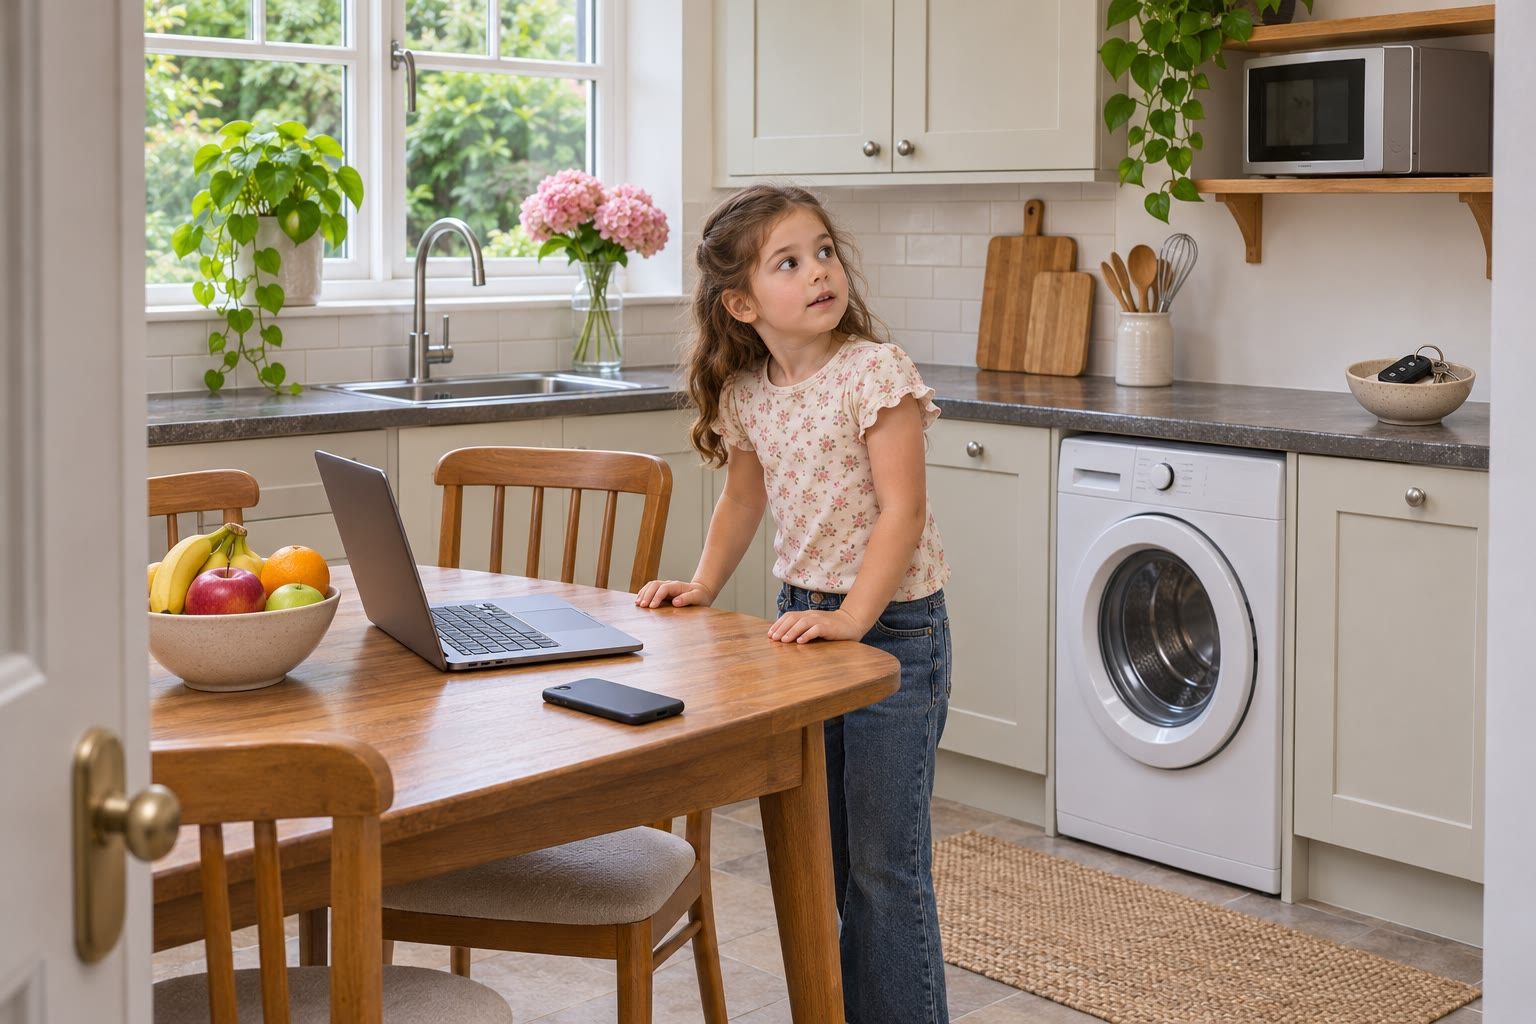
\includegraphics[width=0.66\linewidth]{images/book1/ai/g1-what-is-a-computer-kitchen.jpg}

{\small A family kitchen. How many \omterm{def:g1:what-is-a-computer:computer}{computers} can you find? Some of them are
hidden inside other machines.}
\end{omfigure}

\section{Computers around us}

Some \omterm{def:g1:what-is-a-computer:computer}{computers} are easy to see. A \emph{desktop \omterm{def:g1:what-is-a-computer:computer}{computer}} stays on a desk,
with a big screen, a keyboard and a mouse. A \emph{laptop} folds shut and can
be carried in a bag. A tablet is a flat screen you touch with your fingers. A
phone is a small \omterm{def:g1:what-is-a-computer:computer}{computer} that also makes calls.

\begin{definition}[Computer]\label{def:g1:what-is-a-computer:computer}
A \emph{computer}\index{computer} is a machine that follows instructions to
work on information: it takes information in, changes it, keeps it, and gives
information back out.
\end{definition}

Many \omterm{def:g1:what-is-a-computer:computer}{computers} are hidden. They are small, and they live inside other
machines: a washing machine, an oven, a car, a lift, a toy that talks, a
traffic light. You never see their screen, because most of them have none.
They are still \omterm{def:g1:what-is-a-computer:computer}{computers}: each one follows its instructions.

\begin{example}[Computers in Mia's kitchen]\label{ex:g1:what-is-a-computer:kitchen}
In Mia's kitchen there are at least five \omterm{def:g1:what-is-a-computer:computer}{computers}: the laptop, the phone, the
washing machine's \omterm{def:g1:what-is-a-computer:computer}{computer}, the oven's \omterm{def:g1:what-is-a-computer:computer}{computer} and the car key's \omterm{def:g1:what-is-a-computer:computer}{computer}.
Only two of them have a screen. The bowl, the table and the chairs are not
\omterm{def:g1:what-is-a-computer:computer}{computers}: they follow no instructions at all.
\end{example}

\begin{omfigure}
\begin{tikzpicture}[x=1cm, y=1cm, font=\small]
  % desktop computer
  \begin{scope}[shift={(0,0)}]
    \draw[black!70, fill=black!5, rounded corners=2pt] (0,1.2) rectangle (3.2,3.4);
    \fill[ocPaleBlue] (0.15,1.35) rectangle (3.05,3.25);
    \draw[black!70, fill=black!15] (1.4,0.75) rectangle (1.8,1.2);
    \draw[black!70, fill=black!15] (0.9,0.6) rectangle (2.3,0.75);
    \draw[black!70, fill=black!5, rounded corners=1pt] (-0.1,-0.2) rectangle (2.6,0.35);
    \foreach \x in {0.05,0.3,...,2.4} \draw[black!40] (\x,0.0) rectangle ++(0.17,0.17);
    \draw[black!70, fill=black!5] (3.15,0.05) ellipse (0.2 and 0.3);
    \draw[black!70] (3.15,0.35) -- (3.15,0.05);
    \draw[black!50] (2.6,0.1) .. controls (2.8,0.6) .. (3.15,0.35);
    \node[font=\small\bfseries] at (1.6,-0.7) {desktop computer};
    \draw[black!60] (3.25,2.9) -- (3.9,2.9) node[right] {screen};
    \draw[black!60] (1.2,0.35) -- (1.2,0.55) -- (-0.4,0.55) node[left] {keyboard};
    \draw[black!60] (3.35,0.05) -- (3.9,0.05) node[right] {mouse};
  \end{scope}
  % laptop
  \begin{scope}[shift={(7.2,0)}]
    \draw[black!70, fill=black!5, rounded corners=2pt] (0,0.55) -- (0.25,2.9) -- (3.25,2.9) -- (3.5,0.55) -- cycle;
    \fill[ocPaleBlue] (0.4,0.8) -- (0.6,2.7) -- (2.9,2.7) -- (3.1,0.8) -- cycle;
    \draw[black!70, fill=black!10, rounded corners=1pt] (-0.4,-0.2) -- (0,0.55) -- (3.5,0.55) -- (3.9,-0.2) -- cycle;
    \foreach \x in {0.2,0.5,...,3.2} \draw[black!40] (\x,0.25) rectangle ++(0.2,0.15);
    \draw[black!50] (1.35,-0.12) rectangle (2.15,0.15);
    \fill[black!60] (1.75,2.8) circle (0.04);
    \node[font=\small\bfseries] at (1.75,-0.7) {laptop};
    \draw[black!60] (1.75,2.83) -- (1.75,3.3) node[above] {camera};
    \draw[black!60] (2.15,0.0) -- (4.3,0.0) node[right] {touchpad};
    \draw[black!60] (3.2,2.0) -- (4.3,2.0) node[right] {screen};
  \end{scope}
\end{tikzpicture}

{\small Two \omterm{def:g1:what-is-a-computer:computer}{computers} that are easy to see: a desktop \omterm{def:g1:what-is-a-computer:computer}{computer}, with its
screen, keyboard and mouse, and a laptop, which folds shut.}
\label{fig:g1:what-is-a-computer:two-computers}
\end{omfigure}

\section{A machine that follows instructions}

What do all these \omterm{def:g1:what-is-a-computer:computer}{computers} have in common? Each of them follows
instructions. People write the instructions, and the \omterm{def:g1:what-is-a-computer:computer}{computer} carries them
out exactly, one after the other.

A \omterm{def:g1:what-is-a-computer:computer}{computer} is very fast: it can carry out many millions of instructions in
one second. It never gets tired and never gets bored. But it does nothing
else than what its instructions say. If the instructions say ``stop the drum
after one hour'', the washing machine's \omterm{def:g1:what-is-a-computer:computer}{computer} stops the drum after one
hour, even if the clothes are still dirty.

\begin{remark}[A computer does not think for us]\label{rem:g1:what-is-a-computer:exactly}
When a \omterm{def:g1:what-is-a-computer:computer}{computer} does something surprising, it is still following its
instructions. Somebody wrote them, and maybe made a mistake. Finding and
fixing such mistakes is part of the work of the people who write
instructions for \omterm{def:g1:what-is-a-computer:computer}{computers}.
\end{remark}

\begin{history}[The first computers filled a room]
% ledger: g1:eniac-1946, g1:eniac-size, g1:eniac-tubes, g1:eniac-programming
One of the first electronic \omterm{def:g1:what-is-a-computer:computer}{computers} was shown to the public in 1946. It was
called ENIAC. It filled a whole room, about 9 metres by 15 metres, and weighed
about 27 tonnes. It had 18\,000 glass valves that lit up and grew warm. To give
it new instructions, its operators plugged cables in and set switches by hand.
Today a phone is millions of times faster and fits in a pocket.
\end{history}

\begin{omfigure}
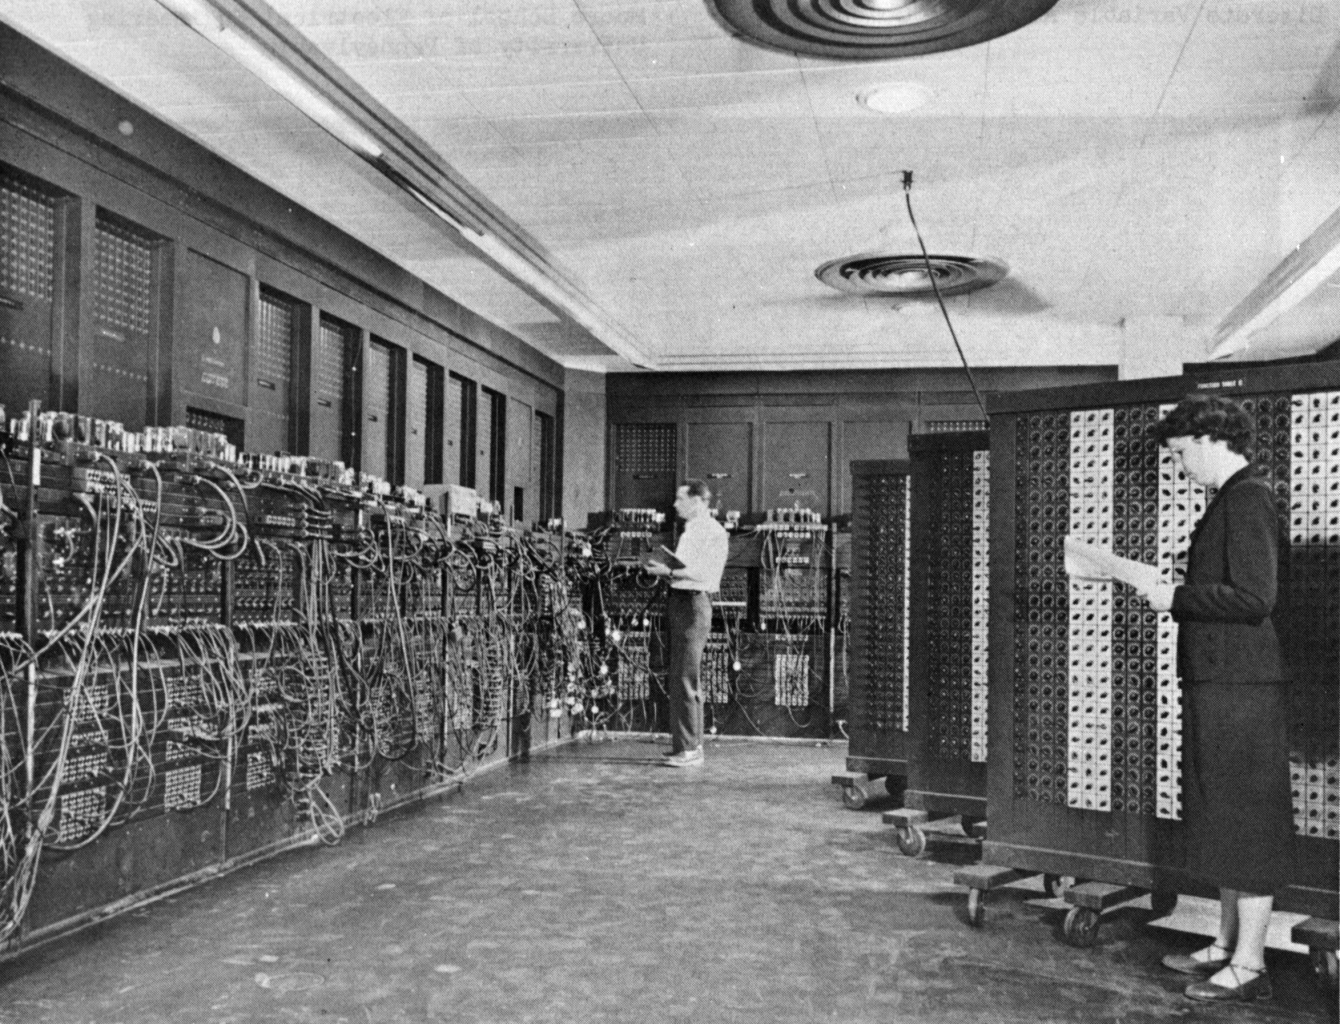
\includegraphics[width=0.62\linewidth]{images/book1/g1-eniac.jpg}

{\small ENIAC, one of the first electronic \omterm{def:g1:what-is-a-computer:computer}{computers}. Two of its operators,
Glen Beck and Betty Snyder, are giving it new instructions. U.S. Army
photograph, public domain.}
\end{omfigure}

\section{What goes in and what comes out}

A \omterm{def:g1:what-is-a-computer:computer}{computer} works on information. Information goes in, the \omterm{def:g1:what-is-a-computer:computer}{computer} works on
it, and information comes out.

\begin{definition}[Input and output]\label{def:g1:what-is-a-computer:input}
The \emph{input}\index{input} of a \omterm{def:g1:what-is-a-computer:computer}{computer} is the information that goes into
it: a key pressed, a click, a word spoken, a photo taken. The
\emph{output}\index{output} of a \omterm{def:g1:what-is-a-computer:computer}{computer} is the information that comes out
of it: letters on a screen, a sound, a picture, a printed page, a motor that
turns.
\end{definition}

\begin{omfigure}
\begin{tikzpicture}[x=1cm, y=1cm, font=\small,
    box/.style={draw=black!70, rounded corners=3pt, minimum height=8mm, align=center, inner sep=3pt},
    arr/.style={-{Stealth[length=2.5mm]}, thick, black!70}]
  \node[font=\bfseries] at (0,3.2) {input};
  \node[font=\bfseries] at (4.5,3.2) {the computer};
  \node[font=\bfseries] at (9,3.2) {output};
  \foreach \y/\i/\c/\o in {2.2/{Mia presses\\the key M}/{laptop}/{the letter M\\appears on the screen},
                          1.0/{Tom clicks on\\a song}/{tablet}/{the song plays\\in the speakers},
                          -0.2/{Dad turns the dial\\to ``cotton''}/{washing machine's\\computer}/{the drum turns\\and water comes in}} {
    \node[box, fill=ocMint!20, text width=3cm] (i) at (0,\y) {\i};
    \node[box, fill=ocPaleBlue, text width=2.8cm] (c) at (4.5,\y) {\c};
    \node[box, fill=ocYellow!30, text width=3.2cm] (o) at (9,\y) {\o};
    \draw[arr] (i) -- (c);
    \draw[arr] (c) -- (o);
  }
\end{tikzpicture}

{\small Information goes in, the \omterm{def:g1:what-is-a-computer:computer}{computer} works on it, and information comes
out. Three examples.}
\label{fig:g1:what-is-a-computer:input-output}
\end{omfigure}

\begin{example}[The washing machine]\label{ex:g1:what-is-a-computer:washing}
The washing machine's \omterm{def:g1:what-is-a-computer:computer}{computer} has several \omterm{def:g1:what-is-a-computer:input}{inputs}. One is the turn of the dial
that chooses the kind of wash. Another is the level of the water in
the drum, which the machine measures by itself. Its \omterm{def:g1:what-is-a-computer:input}{outputs} are the motor that
turns the drum, the tap that lets water in, and a little beep at the end.
\end{example}

\section{The parts we can see and touch}

A \omterm{def:g1:what-is-a-computer:computer}{computer} is connected to the things we use to talk to it and to the things
it uses to answer us.

\begin{definition}[Input device and output device]\label{def:g1:what-is-a-computer:device}
An \emph{input device}\index{input device} is a part that brings \omterm{def:g1:what-is-a-computer:input}{input} into a
\omterm{def:g1:what-is-a-computer:computer}{computer}: a keyboard, a mouse, a touchpad, a microphone, a camera. An
\emph{output device}\index{output device} is a part that takes \omterm{def:g1:what-is-a-computer:input}{output} out of
a \omterm{def:g1:what-is-a-computer:computer}{computer}: a screen, a speaker, headphones, a printer.
\end{definition}

Some parts do both jobs. A touch screen shows pictures, so it is an \omterm{def:g1:what-is-a-computer:device}{output
device}; when you touch it, it tells the \omterm{def:g1:what-is-a-computer:computer}{computer} where your finger is, so it is
also an \omterm{def:g1:what-is-a-computer:device}{input device}. A headset with a microphone is the same: the speakers
are \omterm{def:g1:what-is-a-computer:input}{output}, the microphone is \omterm{def:g1:what-is-a-computer:input}{input}.

\begin{omfigure}
\begin{tikzpicture}[x=1cm, y=1cm, font=\small,
    dev/.style={draw=black!60, rounded corners=3pt, minimum width=2.9cm, minimum height=7mm}]
  \node[font=\bfseries] at (0,4.3) {input devices};
  \node[font=\bfseries] at (4.6,4.3) {output devices};
  \node[font=\bfseries] at (9.2,4.3) {both};
  \foreach \t [count=\k] in {keyboard, mouse, touchpad, microphone, camera}
    \node[dev, fill=ocMint!20] at (0,4.3-0.8*\k) {\t};
  \foreach \t [count=\k] in {screen, speaker, headphones, printer}
    \node[dev, fill=ocYellow!30] at (4.6,4.3-0.8*\k) {\t};
  \node[dev, fill=ocPaleBlue] at (9.2,3.5) {touch screen};
  \node[dev, fill=ocPaleBlue, align=center, minimum height=11mm] at (9.2,2.5) {headset with\\a microphone};
  \draw[black!30] (2.3,4.6) -- (2.3,0); \draw[black!30] (6.9,4.6) -- (6.9,0);
\end{tikzpicture}

{\small Sorting the parts of a \omterm{def:g1:what-is-a-computer:computer}{computer}: \omterm{def:g1:what-is-a-computer:device}{input devices}, \omterm{def:g1:what-is-a-computer:device}{output devices}, and
devices that do both.}
\label{fig:g1:what-is-a-computer:sorting}
\end{omfigure}

\begin{omfigure}
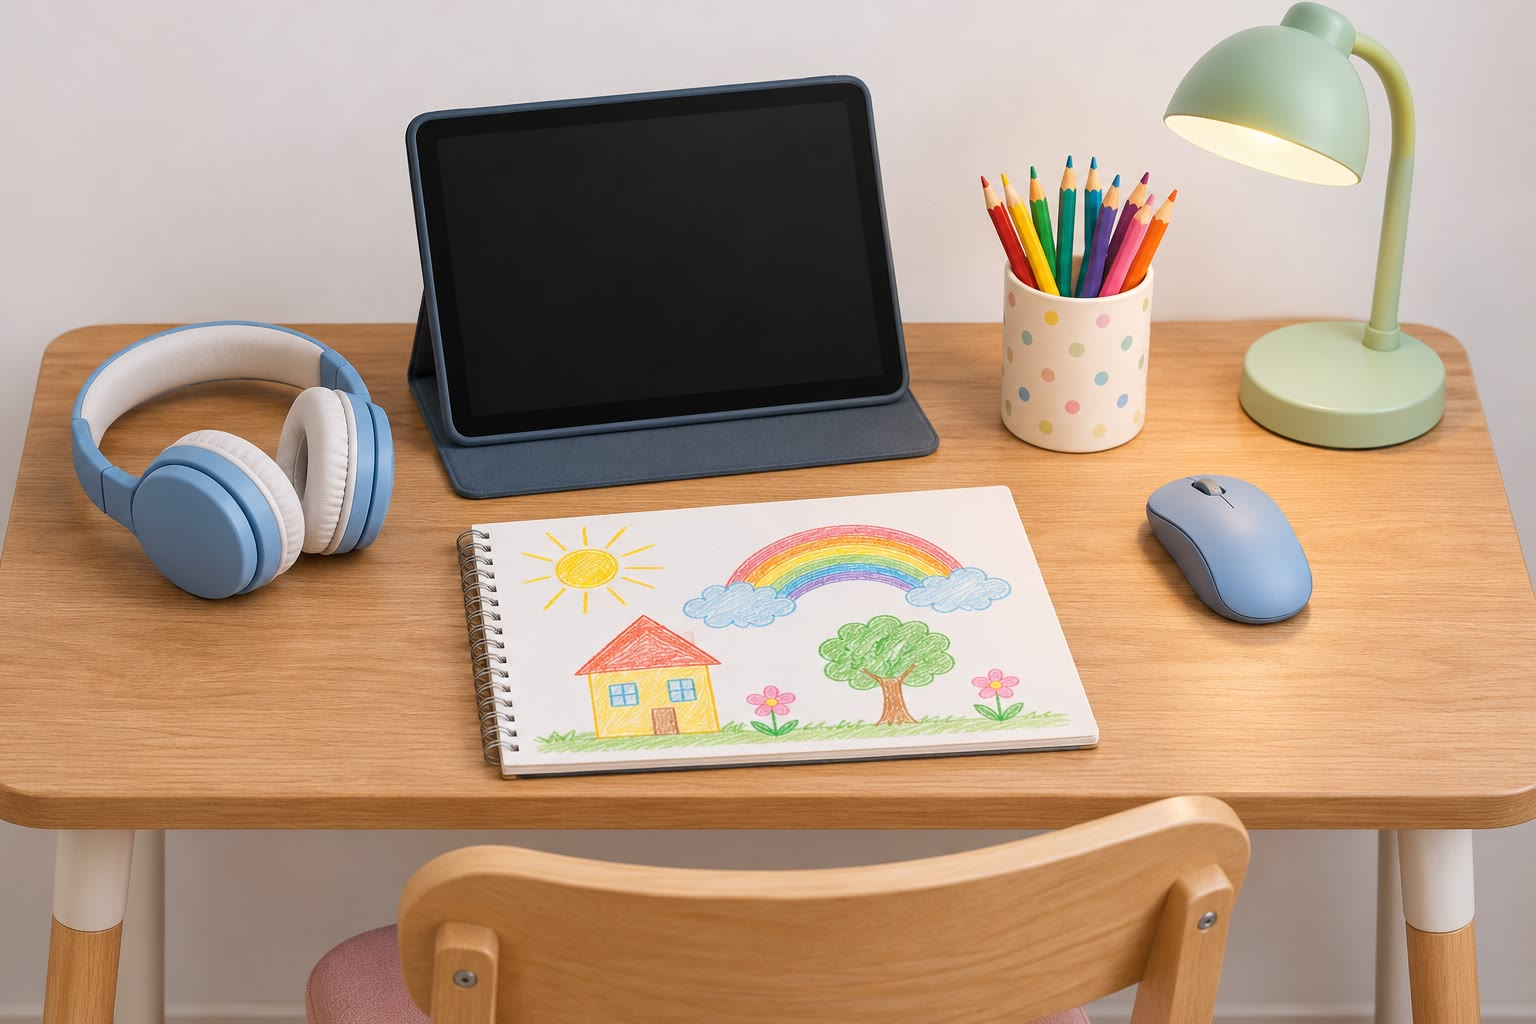
\includegraphics[width=0.6\linewidth]{images/book1/ai/g1-what-is-a-computer-devices.jpg}

{\small A desk with a tablet, headphones and a mouse. Which ones are \omterm{def:g1:what-is-a-computer:device}{input
devices}, and which are \omterm{def:g1:what-is-a-computer:device}{output devices}?}
\end{omfigure}

\section{Exercises}

\begin{exercise}[$\star$]\label{exo:g1:what-is-a-computer:1}
Which of these objects contain a \omterm{def:g1:what-is-a-computer:computer}{computer}? A lamp with a plain switch, a
phone, an oven that stops by itself after the cooking time, a wooden chair, a
car.
\end{exercise}

\begin{exercise}[$\star$]\label{exo:g1:what-is-a-computer:2}
\omterm{def:g1:what-is-a-computer:device}{Input device} or \omterm{def:g1:what-is-a-computer:device}{output device}? A keyboard, a screen, a mouse, a printer, a
microphone, a speaker, a camera, headphones.
\end{exercise}

\begin{exercise}[$\star$]\label{exo:g1:what-is-a-computer:3}
Lina takes a photo with a tablet, and the photo appears on its screen. What is
the \omterm{def:g1:what-is-a-computer:input}{input}? What is the \omterm{def:g1:what-is-a-computer:input}{output}?
\end{exercise}

\begin{exercise}[$\star$]\label{exo:g1:what-is-a-computer:4}
Why is a touch screen both an \omterm{def:g1:what-is-a-computer:device}{input device} and an \omterm{def:g1:what-is-a-computer:device}{output device}?
\end{exercise}

\begin{exercise}[$\star$]\label{exo:g1:what-is-a-computer:5}
Look at the drawing of the desktop \omterm{def:g1:what-is-a-computer:computer}{computer} and the laptop. Name three parts
of the desktop \omterm{def:g1:what-is-a-computer:computer}{computer} and two parts of the laptop.
\end{exercise}

\begin{exercise}[$\star$]\label{exo:g1:what-is-a-computer:6}
Name three \omterm{def:g1:what-is-a-computer:computer}{computers} you could find in a school.
\end{exercise}

\begin{exercise}[$\star$]\label{exo:g1:what-is-a-computer:7}
Tom says: ``A \omterm{def:g1:what-is-a-computer:computer}{computer} always has a screen.'' Is he right? Give an example.
\end{exercise}

\begin{exercise}[$\star$]\label{exo:g1:what-is-a-computer:8}
Sami speaks to a phone: ``Play my favourite song.'' The song plays. What is
the \omterm{def:g1:what-is-a-computer:input}{input}, what is the \omterm{def:g1:what-is-a-computer:input}{output}, and which devices are used?
\end{exercise}

\begin{exercise}[$\star\star$]\label{exo:g1:what-is-a-computer:9}
A pocket calculator: you press keys and the answer appears on a small screen.
Is it a \omterm{def:g1:what-is-a-computer:computer}{computer}? Explain with the words ``follows instructions'', ``\omterm{def:g1:what-is-a-computer:input}{input}''
and ``\omterm{def:g1:what-is-a-computer:input}{output}''.
\end{exercise}

\begin{exercise}[$\star\star$]\label{exo:g1:what-is-a-computer:10}
Name two \omterm{def:g1:what-is-a-computer:input}{inputs} and two \omterm{def:g1:what-is-a-computer:input}{outputs} of a washing machine's \omterm{def:g1:what-is-a-computer:computer}{computer}.
\end{exercise}

\begin{exercise}[$\star\star$]\label{exo:g1:what-is-a-computer:11}
Invent a toy robot that rolls on the floor and stops when it touches a wall.
What goes into its \omterm{def:g1:what-is-a-computer:computer}{computer}? What comes out?
\end{exercise}
